\title{Syllabus for Calculus-Based Physics II: Electricity and Magnetism (PHYS180)}
\author{Dr. Jordan Hanson - Whittier College Dept. of Physics and Astronomy}
\date{\today}
\documentclass[10pt]{article}
\usepackage[margin=1.5cm]{geometry}
\usepackage{outlines}
\usepackage{hyperref}
\usepackage{graphicx}
\begin{document}
\maketitle

\begin{abstract}
The concepts of calculus-based electromagnetism will be presented within the context of interactive problem-solving.  The course will begin with the concepts of electric charge, electrostatics, electric potential, and capacitance.  Next, current and DC circuits will be covered.  Magnetostatics and magnetic induction follow DC circuits, concluding with AC circuits.  Finally, seleted topics in electromagnetic waves and optics will be presented.  The course work will include interactive computational exercises, analytic textbook problems, group-designed projects, and lab-based activities.
\end{abstract}
\noindent
\textit{\textbf{Pre-requisites}: PHYS150 or PHYS135A, MATH142 (may be taken concurrently)} \\
\textit{\textbf{Course credits, Liberal Arts Categorization}: 4 Credits, NSIN, QR2} \\
\textit{\textbf{Regular course hours and location}: MWF - 13:30-14:50, SLC 228.} \\
\textit{\textbf{Instructor contact information}: Discord: 918particle, Email: jhanson2@whittier.edu, Office: SLC 222.} \\
\noindent
\textit{\textbf{Office hours}: Book online appointments: \url{https://calendar.app.google/xjeWMYHSuuWvEYKMA}.} \\
\textit{\textbf{Attendance/Absence}: Students needing to reschedule midterms must notify the professor a few days in advance.} \\ 
\textit{\textbf{Late work policy}: Late work is generally not accepted, but is left to the discretion of the instructor.} \\
\textit{\textbf{Text}: University Physics, vol. 2: \url{https://openstax.org/details/books/university-physics-volume-2}.} \\
\textit{\textbf{Homework}: Homework exercises and content will be managed by ExpertTA.  This online system costs \$35 and will provide hints, feedback, and automatically grade student work.  Please click this link to register: \url{https://reg.theexpertta.com/USB06CA-080799-4T2}.} \\
\textit{\textbf{Grading}: The course grade will be a weighted average of assignment scores, and the weights are listed in Tab. \ref{tab:grades}.}
\begin{table}
\centering
\begin{tabular}{| c | c | c |}
\hline
\textbf{Assignment} & \textbf{Weight} & \textbf{Date} \\ \hline
Daily exercises & 10 \% & Completed during class\\ \hline
Homework sets and labs & 30 \% & Weekly on Fridays \\ \hline
First Midterm & 20 \% & March 9th, 2026 (take-home style on Units 0-2)\\ \hline
Second Midterm & 20 \% & May 4th, 2026 (take-home style on Units 3-5) \\ \hline
Final Project Presentation & 20 \% & April 27th and 29th, 2026 (in class) \\ \hline
\end{tabular}
\caption{\label{tab:grades} Grade weighting. The final project presentation may be given via \textbf{Option A} or \textbf{Option B} (see below).}
\end{table} \\
\noindent
\textit{\textbf{Grade Settings}: $\geq 60\%, <70\%$ = D, $\geq 70\%, <80\%$ = C, $\geq 80\%, <90\%$ = B, $\geq 90\%, <100\%$ = A. Pluses and minuses: 0-3\% minus, 3\%-6\% straight, 6\%-10\% plus (e.g. 79\% = C+, 91\% = A-).} \\
\textit{\textbf{ADA Statement on Disability Services}: Whittier College is committed to make learning experiences as accessible as possible. If you experience physical or academic barriers due to a disability, you are encouraged to contact Student Disability Services (SDS) to discuss options. To learn more about academic accommodations, email disabilityservices@whittier.edu, call (562) 907-4825, or go to SDS which is located on the ground floor of Wardman Library.} \\
\textit{\textbf{Academic Honesty:} \url{https://www.whittier.edu/policies/academic/honesty}} \\
\noindent
\textit{\textbf{Course Objectives}:}
\begin{itemize}
\item To solve word problems in physics and mathematics, to construct mathematical models of systems
\item To match mathematical models of physical systems to experimental results
\item To apply logical thinking to conceptually-posed physics problems
\item To practice using scientific instrumentation, to collect and analyze data, and to communicate results
\item To practice written and oral expression of scientifically technical ideas
\end{itemize}
\twocolumn
\textit{\textbf{Course Outline}:}
\begin{outline}[enumerate]
\1 \textbf{Unit 0:} Review of pre-requisite courses, and electrostatics.
\2 Unit analysis, kinematics, and Newton's Laws
\2 Work and energy, momentum
\2 Electrostatics, I - \textbf{Chapters - 5.1-5.7, 6.1-6.4}
\3 The Coulomb force, Newton's Second Law for electric charge
\3 Electric fields of charge distributions
\3 Guass' Law for charge distributions
\2 Electrostatics, II - \textbf{Chapters 7.1-7.6}
\3 Electric potential and potential energy
\3 Electric potential and fields
\3 Equipotentials and conductors
\3 Applications of electrostatics
\1 \textbf{Unit 1:} Capacitors and DC current
\2 Capacitors and capacitance - \textbf{Chapters 8.1-8.4}
\3 Capacitance and capacitors
\3 Series and parallel capacitors, energy considerations
\2 DC current - \textbf{Chapters 9.1-9.5}
\3 Definition of current, Ohm's law
\3 Energy and power in DC current
\1 \textbf{Unit 2:} DC Circuits
\2 DC circuit analysis - \textbf{Chapters 10.1-10.3}
\3 Electromotive force
\3 Resistors in series and parallel
\3 Kirchhoff's rules
\2 Applications - \textbf{Chapters 10.4-10.6}
\3 Instruments to measure current and voltage
\3 RC circuits
\3 Household wiring
\1 \textbf{First Midterm} - due March 9th, 2026.
\2 The midterm will be posted on Moodle on Friday, March 6th.
\2 The exam will be completed at home, with an open-book/open-note policy.  The format includes multiple choice, written exercises, and design problems.
\2 The exam is due in PDF form on Monday, March 9th, to be submitted via Moodle. \\ \\ \\ \\ \\ \\
\1 \textbf{Unit 3:} Magnetism I
\2 Magnetostatics I - \textbf{Chapters 11.1-11.7}
\3 Lorentz force and magnetic field lines
\3 Motion of free charge in magnetic fields
\3 Force on current-carrying conductors
\3 The Hall effect
\2 Magnetostatics II - \textbf{Chapters 12.1-12.7}
\3 Biot-Savart law
\3 Amp\`{e}re's Law: magnetic fields created by current
\1 \textbf{Unit 4:} Magnetism II
\2 Magnetic induction - \textbf{Chapters 13.1-13.7}
\3 Faraday and Lenz's laws
\3 Motional emf
\3 Induced E-fields
\3 Applications of induction
\2 AC circuits - \textbf{Chapters 14.1-14.6, 15.1-15.3}
\3 Mutual and self-inductance
\3 Energy considerations
\3 RL circuits
\3 RLC circuits
\1 \textbf{Unit 5:} AC Circuits and Electromagnetic Waves
\2 AC circuits - \textbf{Chapters 15.1-15.6}
\3 AC sources and circuits
\3 RLC series circuits
\3 Power in AC circuits
\2 Electromagnetic waves - \textbf{Chapters 16.1-16.3}
\3 Maxwell's equations
\3 Electromagnetic plane waves
\3 Energy and momentum considerations
\1 \textbf{Second midterm} - due May 4th, 2026.
\2 The midterm will be posted on Moodle on Friday, May 1st.
\2 The exam will be completed at home, with an open-book/open-note policy.  The format includes multiple choice, written exercises, and design problems.
\2 The exam is due in PDF form on Monday, May 4th, to be submitted via Moodle. \\ \\ \\ \\ \\ \\ \\ \\ \\
\1 \textbf{Final project presentations}
\2 Given on April 27th and 29th, teams of 1-3
\2 Project is a self-designed physics experiment
\2 \textbf{Option A}: A 10-15 minute traditional presentation with several minutes for questions.
\2 \textbf{Option B}: A video in digital storytelling format using WeVideo, also 10-15 minutes long.
\2 Students will receive training and access for the WeVideo tools, which Whittier College provides for free.
\2 Presentations will be graded according to the following breakdown:
\3 For presenting results emphasizing \textit{precision and attention to detail}, with \textit{experimentally verifiable} content, 30\%.
\3 For \textit{clearly communicating} the content, including legibility and sensible graphics, 30\%.
\3 For \textit{meeting but not exceeding} the time-requirement with appropriate amount of content, 30\%.
\3 For \textit{articulating the idea with a unique style}, 10\%.
\end{outline}
\begin{figure}
\centering
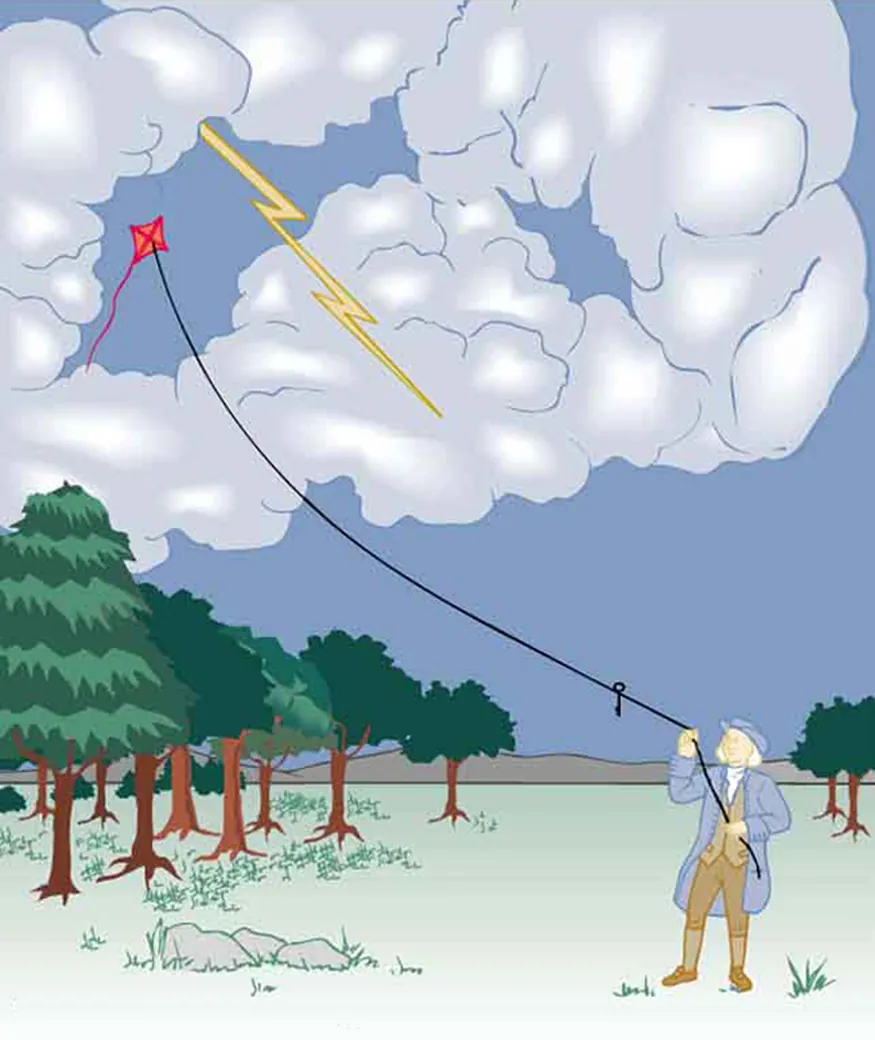
\includegraphics[width=0.25\textwidth]{figures/franklin.png}
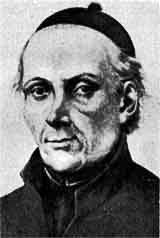
\includegraphics[width=0.2\textwidth]{figures/alzate_ramirez.jpg} \\
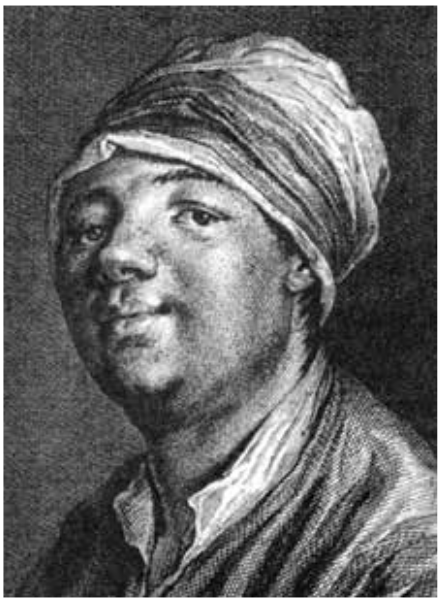
\includegraphics[width=0.23\textwidth]{figures/Abbot_dAuteroche.png}
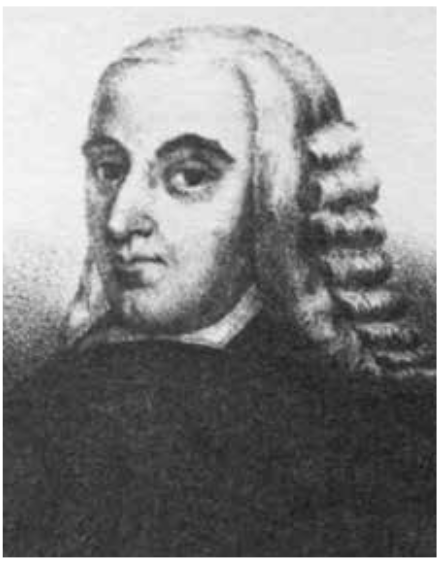
\includegraphics[width=0.24\textwidth]{figures/joaquin_v_d_Leon.png}
\caption{\label{fig:franklin} \small (Top left) Benjamin Franklin, (Top right) Father Jos\'{e} Antonio Alzate y Ram\'{i}rez. (Bottom left) Jean-Baptiste Chapp\'{e} d'Auteroche, (Bottomi right) Joaqu\'{i}n Vel\'{a}zquez de Le\'{o}n.}
\end{figure}
%\begin{figure}
%\centering
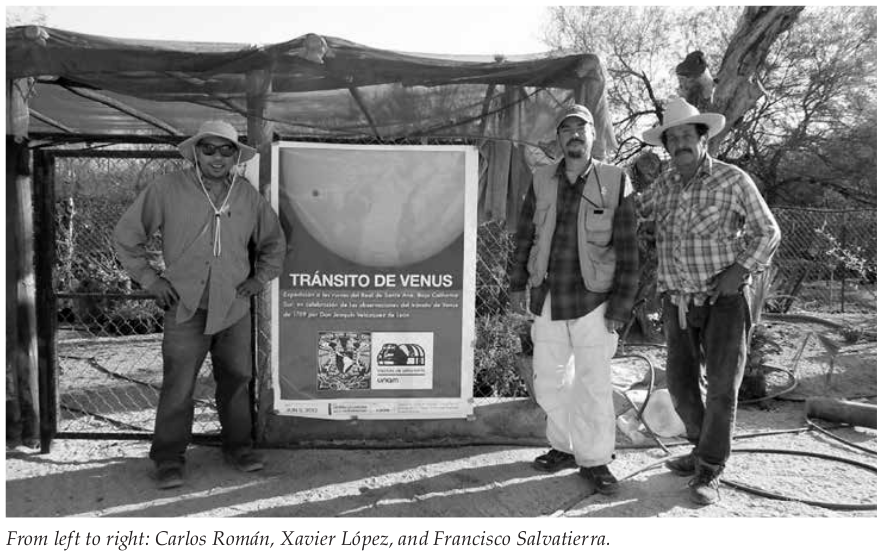
\includegraphics[width=0.45\textwidth]{figures/roman_lopez_salvatierra.png} \\
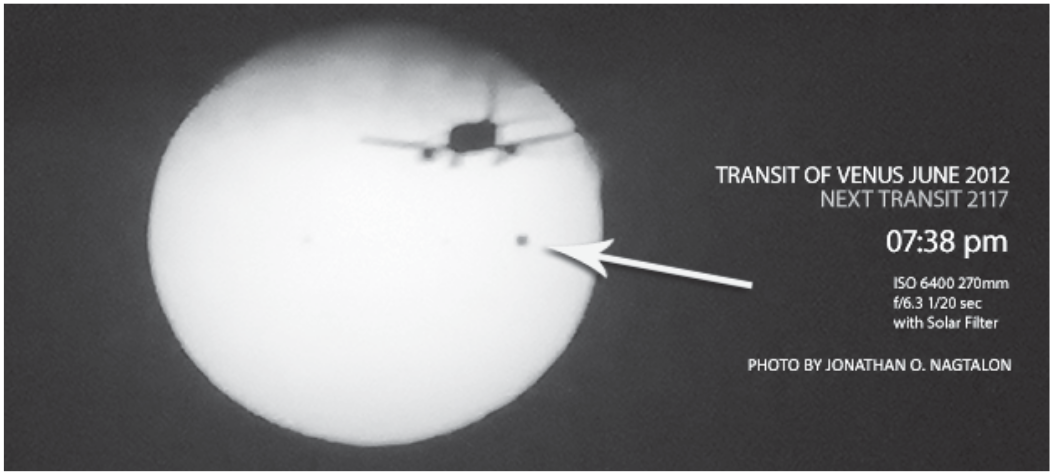
\includegraphics[width=0.45\textwidth]{figures/venus.png} \\
\small Figure 2: (Top) Carlos Rom\'{a}n, Xavier L\'{o}pez, and Fransisco \\ Salvatierra. (Bottom) The 2012 Venus transit, from Baja \\ California.
%\caption{\label{fig:franklin2} \small (Top) Carlos Rom\'{a}n, Xavier L\'{o}pez, and Fransisco Salvatierra. (Bottom) The 2012 Venus transit, from Baja California.}
%\end{figure}
\end{document}
